\documentclass[12pt, letterpaper]{memoir}
\usepackage{NotesStyle}
\geometry{margin=0.75in}

\begin{document}
	\mainmatter
	
	\begin{center}
		{\Huge CHEM 3620}
		{\LARGE-- Exam 1 Equations}
		\begin{description}
			\item[Q:] How would a chemist determine the correct amount of quacamole to put on her burrito?
		\end{description}
	
		
		\begin{center}
			\begin{equation*}
				\hat{H}\psi = -\dfrac{\hbar^2}{2m}\nabla^2\psi + V\psi = E\psi
			\end{equation*}
		
		
			\begin{minipage}[c]{0.7\textwidth}
				\begin{mdframed}
					\centering
					Spherical Polar Coordinates
					\hrule
					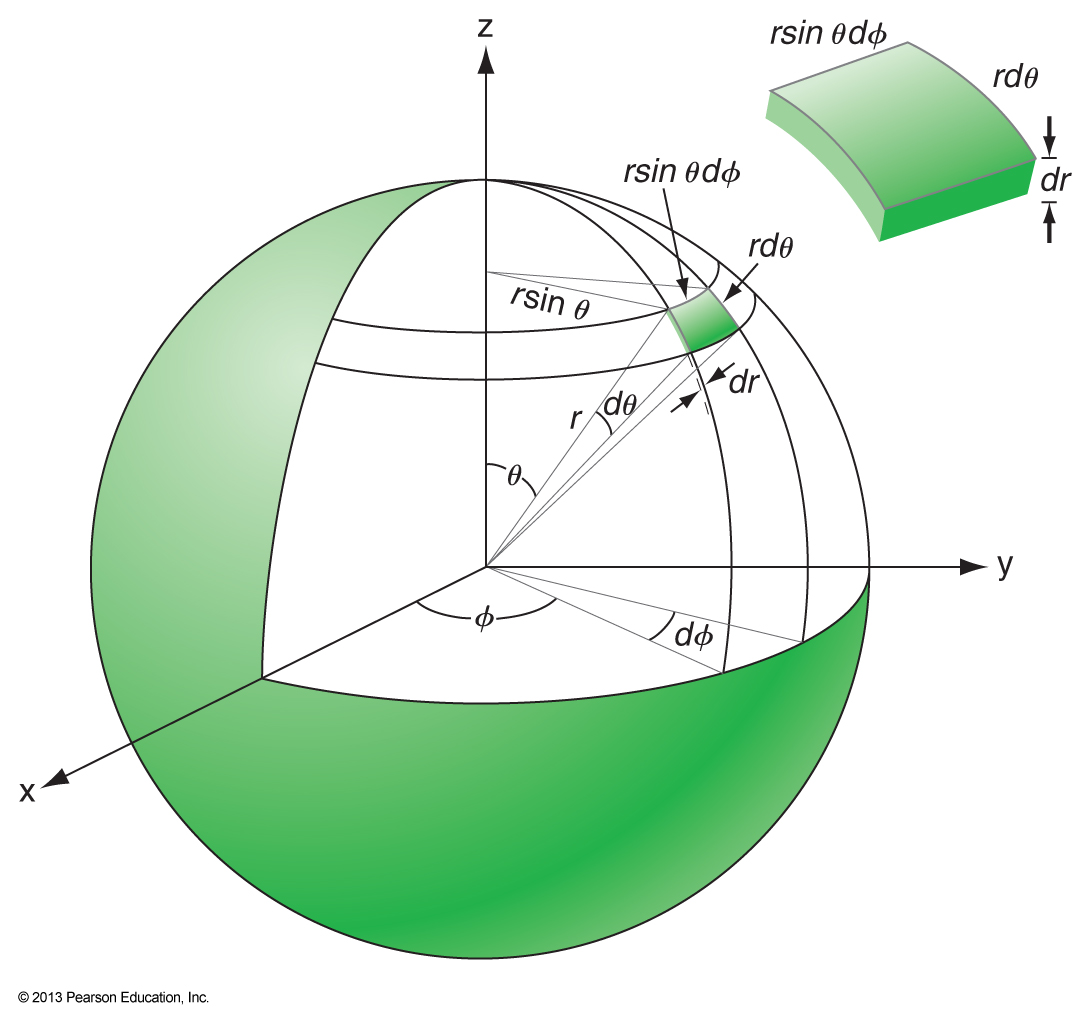
\includegraphics[width = \textwidth]{02_05_Figure}
				\end{mdframed}
			\end{minipage}
		\end{center}

	
		
		\begin{tabular}{ccrl}
			\multicolumn{4}{c}{Table of Particle Properties}\\
			\toprule
			Name&Symbol&\multicolumn{1}{c}{Value}&\multicolumn{1}{c}{Units}\\
			\midrule
			\midrule
			Elementary Charge		& $e$		& $1.602177\times10^{-19}$	& $C$\\
			\midrule
			Electron Rest-Mass		& $m_e$		& $9.109382\times10^{-31}$	& $kg$\\
			\midrule
			Proton Rest-Mass		& $m_p$		& $1.672622\times10^{-27}$	& $kg$\\
			\midrule
			Neutron Rest-Mass		& $m_n$		& $1.674927\times10^{-27}$	& $kg$\\
			\bottomrule
		\end{tabular}

		\begin{description}
			\item[A:] She would use Avocado's number! -- Good luck!
		\end{description}
		
				
	\end{center}
	
	\newpage

		\begin{minipage}{0.495\textwidth}			
			\begin{equation*}
			\lambda=\frac{h}{mv}
			\end{equation*}
			
			\begin{equation*}
			\displaystyle\int_{0}^{\infty}\displaystyle\int_{0}^{\pi}\displaystyle\int_{0}^{2\pi}\psi^{*}\psi r^2\sin\theta\mathrm{d}\phi\mathrm{d}\theta\mathrm{d}r=1
			\end{equation*}			

			
			\begin{equation*}
			\Delta p_x\Delta x \geq \frac{1}{2}\hbar
			\end{equation*}
		
			\begin{equation*}
			\kappa = \dfrac{\sqrt{2m(V-E)}}{\hbar}
			\end{equation*}
		
			\begin{equation*}
			\epsilon = \dfrac{E}{V}
			\end{equation*}
		
			\begin{equation*}
			T=\left[1+\frac{\left(e^{\kappa L} - e^{-\kappa L}\right)^2}{16\epsilon(1-\epsilon)}\right]^{-1}
			\end{equation*}
			
			\begin{equation*}
				\Psi_k(x) = Ae^{ikx} + Be^{-ikx}	
			\end{equation*}
			
			\begin{equation*}
				E_k = \frac{k^2\hbar^2}{2m}
			\end{equation*}
			
			\begin{equation*}
			\psi_n(x) = \sqrt{\dfrac{2}{L}}\sin\left(\dfrac{n\pi x}{L}\right)
			\end{equation*}			
		
		
		\end{minipage}
		\begin{minipage}{0.495\textwidth}	
			\begin{equation*}
			\hat{p}_x = \dfrac{\hbar}{i}\dfrac{\mathrm{d}}{\mathrm{d}x}
			\end{equation*}	
			
			\begin{equation*}
			N^{2} \int \phi^*(\tau)\phi(\tau)d\tau = 1
			\end{equation*}
			
			\begin{equation*}
			\int{\phi^*_n(\tau)\phi_m(\tau)d\tau} = 0 ~~~~ \text{for}~n\neq m
			\end{equation*}
			
			\begin{equation*}
				\int{\phi^*_n(\tau)\phi_m(\tau)d\tau} = 1 ~~~~ \text{for}~n = m
			\end{equation*}
			
			\begin{equation*}
			\avg{\hat{A}} = \displaystyle\int\psi^*\hat{A}\psi\mathrm{d}\tau
			\end{equation*}
			
			\begin{equation*}
			\Delta p_x = \left[\avg{p_x^2}-\avg{p_x}^2\right]^{\nicefrac{1}{2}}
			\end{equation*}			
			
			\begin{equation*}
			E_n = \dfrac{n^2h^2}{8mL^2}
			\end{equation*}
			
			\begin{equation*}
				E_{n_x,n_y} = \dfrac{h^2}{8m}\left(\frac{n_x^2}{L_x^2}+\frac{n_y^2}{L_y^2}\right)
			\end{equation*}
			
			\begin{equation*}
				E_{n_x,n_y,n_z} = \dfrac{h^2}{8m}\left(\frac{n_x^2}{L_x^2}+\frac{n_y^2}{L_y^2}+\frac{n_z^2}{L_z^2}\right)
			\end{equation*}		
		\end{minipage}

	\begin{equation*}
		\psi_{n_x,n_y}(x,y) = \dfrac{2}{\sqrt{L_xL_y}}\sin\left(\dfrac{n_x\pi x}{L_x}\right)\sin\left(\dfrac{n_y\pi y}{L_y}\right)
	\end{equation*}

	\begin{equation*}
		\psi_{n_x,n_y,n_z}(x,y,z) = \sqrt{\dfrac{8}{L_xL_yL_z}}\sin\left(\dfrac{n_x\pi x}{L_x}\right)\sin\left(\dfrac{n_y\pi y}{L_y}\right)\sin\left(\dfrac{n_z\pi z}{L_z}\right)
	\end{equation*}

		\begin{minipage}{0.495\textwidth}
		
				
			\begin{equation*}
				\omega=\sqrt{\dfrac{k_f}{\mu}}
			\end{equation*}			
			
			\begin{equation*}
				\psi_v(x) = N_vH_v\left(\dfrac{x}{\alpha}\right)e^{-\dfrac{x^2}{2\alpha^2}}
			\end{equation*}
		
			\begin{equation*}
				\Psi_{m_l}(\phi)=\frac{e^{im_l\phi}}{\sqrt{2\pi}}
			\end{equation*}
			
			\begin{equation*}
				E_{m_l}=\frac{m_l^2\hbar^2}{2I}
			\end{equation*}
			
			\begin{equation*}
				I=mr^2
			\end{equation*}
		
			\begin{equation*}
				E_{l,m_l}=l(l+1)\dfrac{\hbar^2}{2I}
			\end{equation*}
			
			\begin{equation*}
				\hat{l}^2\psi=l(l+1)\hbar^2\psi
			\end{equation*}		
		
			\begin{equation*}
				h = 6.626\times10^{-34}J~s
			\end{equation*}
					
		\end{minipage}
		\begin{minipage}{0.495\textwidth}	
		
			\begin{equation*}
				E_v = \left(v+\frac{1}{2}\right) \hbar\omega
			\end{equation*}
			
			\begin{equation*}
				\mu=\frac{m_Am_B}{m_A+m_B}
			\end{equation*}
			
			\begin{equation*}
				V(x)=\frac{1}{2}k_fx^2
			\end{equation*}
		
		\begin{equation*}
			\alpha = \left(\dfrac{\hbar^2}{\mu k_f}\right)^{\nicefrac{1}{4}}
		\end{equation*}		
			
			\begin{equation*}
				\Psi_{l,m_l}(\theta, \phi)=Y_l^{m_l}
			\end{equation*}
			
			\begin{equation*}
				m_l = 0, \pm1, \pm2, \ldots \pm l
			\end{equation*}
						
			\begin{equation*}
			\hat{l}_z\psi=m_l\psi
			\end{equation*}
			
			\begin{equation*}
				6.022\times10^{23}AMU=1g
			\end{equation*}
		
			\begin{equation*}
				\hbar = 1.055\times10^{-34}J~s
			\end{equation*}
			
		\end{minipage}
%
%	\begin{mdframed}
%		\centering
%		Useful Integrals and Derivatives\hrule
%		\vspace{-6pt}
%		\begin{minipage}{0.495\textwidth}
%			\begin{equation*}
%			\int_0^\infty x^ne^{-\alpha x}dx = \frac{n!}{\alpha^{n=1}}
%			\end{equation*}
%			
%			\begin{equation*}
%			\int_0^\infty e^{-\alpha x^2}dx = \sqrt{\frac{\pi}{4\alpha}}
%			\end{equation*}
%			
%			\begin{equation*}
%			\int e^{\alpha x}dx =\frac{1}{\alpha}e^{\alpha x} + c
%			\end{equation*}
%			
%			\begin{equation*}
%			\int \sin^2{(\alpha x)}dx =\frac{x}{2}-\frac{\sin{(2\alpha x)}}{4\alpha} + c
%			\end{equation*}
%		\end{minipage}
%		\begin{minipage}{0.495\textwidth}
%			\begin{equation*}
%			\frac{d}{dx}\sin{(\alpha x)} = \alpha\cos{(\alpha x)}
%			\end{equation*}
%			
%			\begin{equation*}
%			\frac{d}{dx}\cos{(\alpha x)} = -\alpha\sin{(\alpha x)}
%			\end{equation*}
%			
%			\begin{equation*}
%			\frac{d}{dx}f(g(x)) = f^\prime(g(x))g^\prime(x)
%			\end{equation*}
%			
%			\begin{equation*}
%			\frac{d}{dx}f(x)g(x) = f^\prime(x)g(x) + f(x)g^\prime(x)
%			\end{equation*}
%		\end{minipage}
%		
%		\vspace{10pt}
%		\begin{equation*}
%		\int x^2\sin{(\alpha x)}dx =\frac{\left(2-\alpha^2x^2\right)\cos(\alpha x)}{\alpha^3} + \frac{2x\sin{(\alpha x)}}{\alpha^2} + c
%		\end{equation*}
%		
%		\begin{equation*}
%		\int x\sin(\alpha x)dx = \frac{\sin(\alpha x) - \alpha x \cos(\alpha x)}{\alpha^2} + c
%		\end{equation*}
%	\end{mdframed}
	

	
%	\begin{table}[htbp]
%		\centering
%		Table of Physical Constants
%		\begin{tabular}{ccrl}
%			\toprule
%			Name&Symbol&\multicolumn{1}{c}{Value}&\multicolumn{1}{c}{Units}\\
%			\midrule
%			\midrule
%			Avogadro's Number 		& $N_{Av}$ 	& $6.022141\times 10^{23}$	& $mol^{-1}$\\
%			\midrule
%			\multirow{2}{*}{Ideal Gas Constant}	& \multirow{2}{*}{$R$} 	& $8.314462$	& $J~mol^{-1}~K^{-1}$\\
%			& 		& $0.08205746$			& $l~atm~mol^{-1}~K^{-1}$\\				
%			\midrule
%			Planck's Constant&$h$	& $6.626070\times10^{-34}$	& $J~s$\\
%			\midrule
%			Reduced $h$	\rule[-10pt]{0pt}{30pt}& $\hbar = \dfrac{h}{2\pi}$	& $1.054572\times10^{-34}$	& $J~s$\\
%			\midrule
%			Boltzmann's Constant	& $k_B$	& $1.380649\times10^{-23}$	& $J~K^{-1}$\\
%			\midrule
%			Faraday's Constant		& $F$		& $96485.34$			& $C~mol^{-1}$\\
%			\midrule
%			Speed of Light	& $c$	& $2.99792458\times10^{8}$	& $m~s^{-1}$\\
%			\midrule
%			Acceleration in Earth's Gravity	& $g$	& $9.80665$			& $m~s^{-2}$\\
%			\midrule
%			Gravitational Constant		& $G$		& $6.67384\times10^{-11}$	& $m^3~kg^{-1}~s^{-2}$\\
%			\midrule
%			Vacuum Permittivity		& $\epsilon_\circ$	& $8.854188\times10^{-12}$	& $F~m^{-1}$\\
%			\midrule
%			Vacuum Permeability &$\mu_\circ = 4\pi\times10^{-7}$  & $1.256637\times10^{-6}$	&$N~A^{-2}$\\
%			\midrule
%			Bohr Radius \rule[-12pt]{0pt}{32pt}& $a_\circ = \dfrac{\epsilon_\circ h^2}{\pi m_e e^2}$ & $5.291772\times10^{-11}$ &$m$\\
%			\midrule		
%			\multirow{2}{*}{Rhydberg Constant for \ch{^1H}} & \multirow{2}{*}{$R_H$} & $2.17869689\times10^{-18}$ & $J$\\
%			& & $109677.581$ & $cm^{-1}$\\
%			\bottomrule
%		\end{tabular}	
%	\end{table}
\end{document}	